\begin{figure}[htbp]
\centering
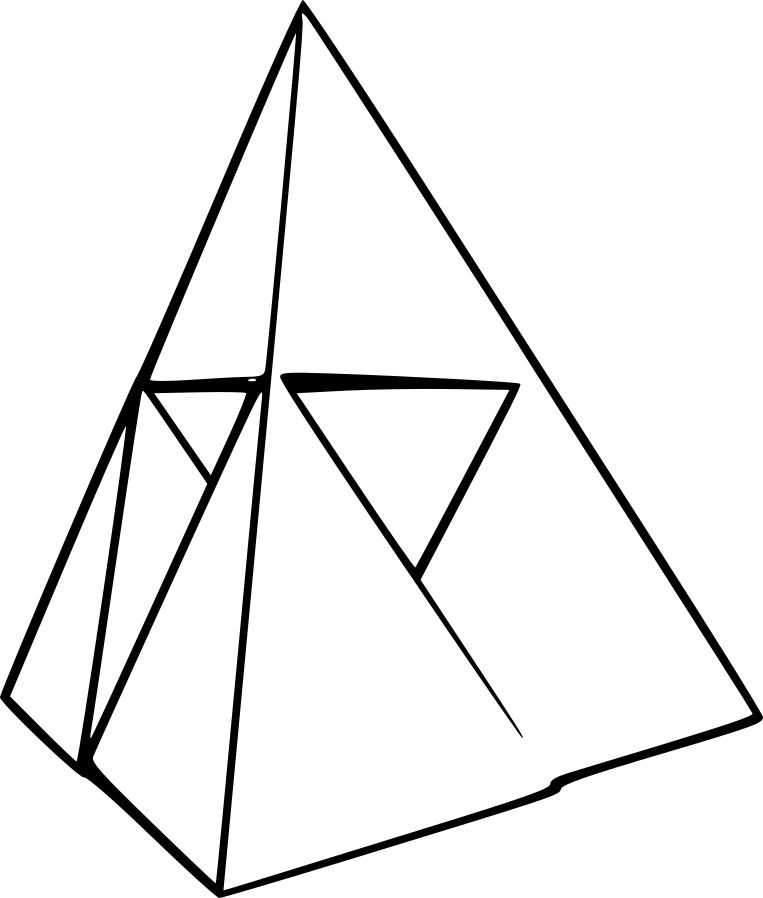
\includegraphics{images/contemplations/contemplation2C.png}
\caption{second Contemplation}
\end{figure}

\subsection{Second Contemplation: Tetrahedral
Fractal}\label{second-contemplation-tetrahedral-fractal}

Sit and look at a free fractal thing in nature while you color this in.
This is symbolizing the fractal nature of truly free things. Trees and
shrubs are all free. Contemplate their fractal nature and their ability
to build this massive structure from the tiny whips of passing carbon
dioxide from the air over many years. Incredible! The tetrahedral
fractal geometry shown in 3d here symbolizes the union of our human
geometry with that of nature.

In this case we flop around on the ground in a more peaceful way, more
slowly, at tai chi speeds even, to try to incorporate the slow pace of
the tree into our thoughts.
